
\documentclass[12pt]{article}
\usepackage[utf8]{inputenc}
\usepackage[T1]{fontenc}
\usepackage[norsk]{babel}
\usepackage{floatpag}				% Different pagestyles
\usepackage{amsmath}
\usepackage{array}	
\usepackage{booktabs}
\usepackage{amssymb}
\usepackage{graphicx}
\usepackage{epstopdf}
\usepackage{tabularx}
\usepackage{float}
\usepackage{caption}
\usepackage{subcaption}
\usepackage{parskip}
\usepackage{multirow}
\usepackage{listings}

\begin{document}
\title{Oblig 7}
\author{Magnus Isaksen}
\maketitle
\newpage 

\section*{Exercises}

\subsection*{a)}

Har van der Waals ligning 

\begin{align*}
(P + \frac{aN^2}{V^2}) (V - Nb) = NkT
\end{align*}

skriver om denne 

\begin{align*}
P + \frac{aN^2}{V^2}) = \frac{NkT}{V-Nb}
\end{align*}

og får 

\begin{align*}
P = \frac{NkT}{V-Nb} - \frac{aN^2}{V^2}
\end{align*}


\subsection*{b)}

Erstatter $P = \hat{P}P_c$ , $V = \hat{V}V_c$ og $T = \hat{T}T_c$


$\hat{P}P_c = \frac{Nk\hat{T}T_c}{\hat{V}V_c - Nb} - \frac{aN^2}{(\hat{V}V_c)^2}$


Setter da inn gitte verdier for $P_c$, $V_c$ og $T_c$

$\hat{P}\frac{a}{27b^2} = \frac{Nk\hat{T} \frac{8a}{27bk}}{\hat{V}3Nb - Nb} - \frac{a^2}{9N^2b^2\hat{V}^2}$

Dermed får vi 

$\hat{P} = \frac{8\hat{T}}{3\hat{V} - 1} - \frac{3}{\hat{V}^2}$

\subsection*{c)}

Lager et program i python som finne trykket som funksjon av volumet. Dette gjør jeg for tre forskjellige temperaturer. 

\begin{lstlisting}

V_hat = linspace(0.4, 20, 200)
T_hat = [1.15, 1.0, 0.85]


P_hat = zeros(200)
P_hat1 = ((8*T_hat[0])/(3*V_hat -1) ) -(3/V_hat**2)
P_hat2 = ((8*T_hat[1])/(3*V_hat -1) ) -(3/V_hat**2)
P_hat3 = ((8*T_hat[2])/(3*V_hat -1) ) -(3/V_hat**2)


#print P_hat1
figure(1)
plot(V_hat,P_hat1, 'b-', V_hat, P_hat2, 'r-', V_hat, P_hat3,'g-')
xlabel('Volume')
ylabel('Pressure')

\end{lstlisting}

Så plotter jeg disse i samme Figur \ref{Fig:volumepressure} og kan se at de avviker fra hverandre rundt volum 1.0, men at de eller ser ut til å holde seg gordt samlet. 

\begin{figure}[ht!] 
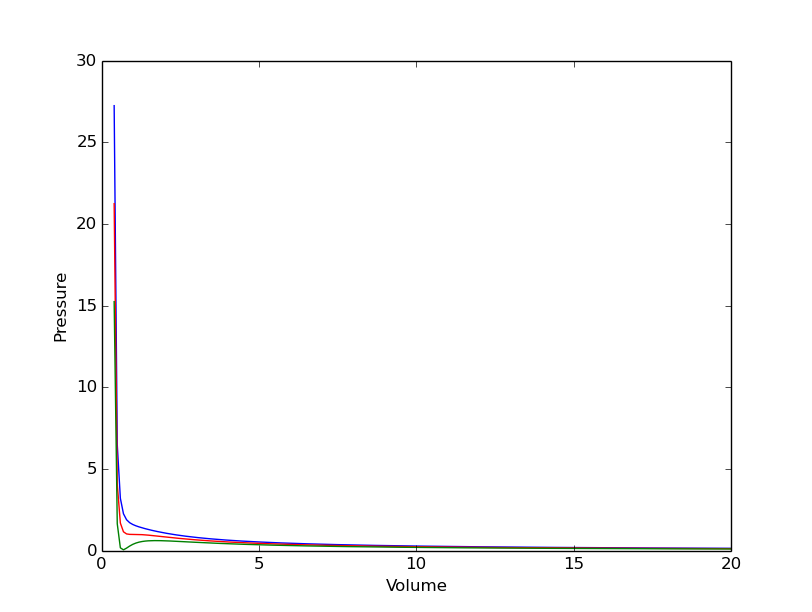
\includegraphics[width = \textwidth]{figure_1.png}
\caption{Trykk som funksjon av volum. Ved T = 1.15, 1.0 og 0.85}
\label{Fig:volumepressure}
\end{figure}

\subsection*{d)}

$\hat{\rho} = \frac{1}{\hat{V} = \frac{\rho}{\rho_c}}$

Setter inn $\hat{\rho}$ for $\frac{1}{\hat{V}}$

og får 

$ \hat{P} = \frac{8\hat{\rho}\hat{T}}{3 - \hat{\rho}} - 3\hat{\rho}$

\subsection*{e)}

Skal nå se på trykk som funksjon av tetthet. Dette blir gjordt ved

\begin{lstlisting}
rho = linspace(0.0,2.0, 200)
P_rho1 = ((8*rho*T_hat[0])/(3-rho))-3*rho**2
P_rho2 = ((8*rho*T_hat[1])/(3-rho))-3*rho**2
P_rho3 = ((8*rho*T_hat[2])/(3-rho))-3*rho**2
figure(2)

plot(rho,P_rho1, rho, P_rho2, rho, P_rho3)
xlabel('rho')
ylabel('Pressure')
\end{lstlisting}

Og får da ut et plot for hver av de tre temperaturene $ T = 0.85, 1.0$ and $1.15$
\begin{figure}[ht!]
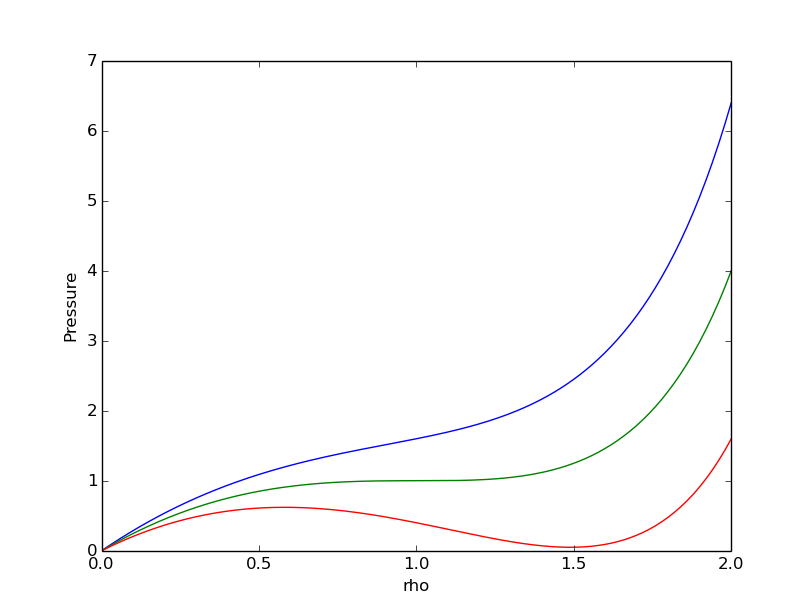
\includegraphics[width = \textwidth]{figure_2.png}
\caption{Pressure as a function of density. Blå linje er T = 1.15, grønn linje er T = 1.0 og rød er T = 0.85}
\label{fig:2}
\end{figure}

\subsection*{f)}

I det den forlater startpunktet blir den unik. Slik at grafene for hver T går fra hverandre. 

\subsection*{g)}

Den blir negativ når stigningstallet til til grafen er nagativ. Dette ser vi skjer når T = 0.85 og med en tetthet på mellom 0.5 og 1.5. 

\subsection*{h)}
Gibbs fri energi er gitt ved 

$G = F + PV$

Hvor F kommer fra Helmholz fri energi og P er trykk og V er volum. 

$F = - NkT(\ln(\frac{n_Q(V -Nb)}{N} + 1) - \frac{aN^2}{V}$

og 

$PV = \frac{VNkT}{V- Nb} - \frac{aN^2}{V}$

Dette gir Gibbs fri energi lik: 

$G = \frac{VNkt}{V - Nb} - NkT(\ln(\frac{n_Q(V-Nb)}{N} + 1) - \frac{2aN^2}{V}$

\subsection*{i)}

Vi har 

$F = - NkT(\ln(\frac{n_Q(V -Nb)}{N}) + 1) - \frac{aN^2}{V}$ og $PV$ oppgitt. 

skriver om $F$ 

$F = - NkT(\ln(\frac{n_Q(V -Nb)}) - \ln(N) + 1) - \frac{aN^2}{V}$

$F = -NkT(\ln(n_Q) + \ln(V-Nb) - \ln(N) + 1) - \frac{aN^2}{V}$ 

$F = -Nkt(\ln(\frac{V- Nb}{N})) - \frac{aN^2}{V} +NkT(\ln(n_Q) +1)$ 

Setter vi dette inn for å finne Gibbs fri energi får vi 

$G = -NkT\ln(\frac{V-Nb}{N}) - \frac{aN^2}{V} + PV  + NkT(\ln(n_Q) +1)$

Hvor det siste leddet er $c(T)$. 

$G = -NkT\ln(\frac{V-Nb}{N}) - \frac{aN^2}{V} + PV  + c(T)$

Her kunne vi fått helt samme uttrykk som oppgaven ber om ved å inkludere $ln(\frac{1}{N})$ inn i $c(T)$. Men fordi jeg fikk hint på datalab om at ved å ha denne med vil neste oppgave bli enklere å få riktig.

\subsection*{j)}

Her skal det inn endel utregninger, gjelder å holde tungen rett i munnen. Noe jeg ikke fikk helt til. Man skal sette inn for T,V, P som i b) og skal også skrive om endel. Brukte kanskje ikke nok tid på dette, men den ble nedprioritert. 

\subsection*{k)}

Lager kode som finner Gibbs fri energi og plotter denne mot trykk i Figur \ref{fig:3}. Også plottes trykk mot tetthet i den øverste, in det midterste plottes trykk som funksjon av volum. 

\begin{lstlisting}
rho = linspace(0.2,2.0, 10000)
T = 0.9
'''
P_rho4 = zeros(len(rho))
g = zeros(len(rho))
'''
jlist = []

P_rho4 = ((8*rho*T)/(3-rho))-3*rho**2
g = -3*rho - (8.0/3.0)*T*log((3.0/rho) -1) + (P_rho4/rho)




for i in range(len(rho)):
    if P_rho4[i] >= 0.499 and P_rho4[i] <= 0.501:
        jlist.append(i)
        
subplot(3,1,1)
plot(rho,P_rho4, 'b-')
xlabel('rho')
ylabel('Pressure')
title('Oblig 7 exercise k')
subplot(3,1,2)
plot(P_rho4, 1/rho,'b-')
xlabel('Pressure')
ylabel('Volume')
subplot(3,1,3)
plot(P_rho4, g,'b-')
xlabel('Pressure')
ylabel('Gibbs free energy')
subplot(3,1,1)
plot(rho[jlist],P_rho4[jlist], 'r*')
subplot(3,1,2)
plot(P_rho4[jlist], 1/rho[jlist], 'r*')
subplot(3,1,3)
\end{lstlisting}

\begin{figure}[ht!]
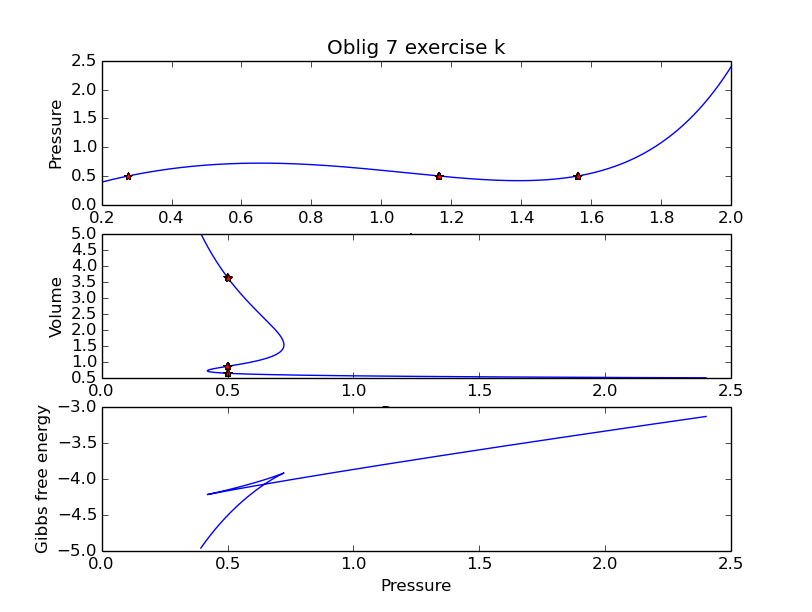
\includegraphics[width = \textwidth]{figure_3.png}
\caption{I øverste Trykk som funksjon av tetthet, in midterste Volum som funksjon av trykk og neders Gibbs fri energi som funksjon av trykk.}
\label{fig:3}
\end{figure}

\subsection*{l)}


Minimum til Gibbs fri energi kan vi finne der grafen krysser seg selv. Dette kan vi gjøre da dette tilsvarer overgangen mellom to tilstander. Og dermed vil dette tilsvare et minimum for den aktuelle tilstanden. Grafen går litt forbi før den øker litt i potensiale i det den bytter tilstand. 


\subsection*{m)}

Da jeg ikke fant en god selfintersect funksjon i python, lagde jeg en test selv. Jeg tror den fungerer, men har ikke sett hvordan det ser ut i matlab, så kan ikke si at testen under fungerer optimalt. Samtidig er den litt treg å kjøre med høy oppløsning.  

\begin{lstlisting}
indexi = []
indexj = []
for i in range(len(g)-1): 
    for j in range(i+1,len(g)): 
        if g[i] >= g[j]-0.00000001 and g[i] <= g[j] + 0.00000001: 
           indexi.append(i)
           indexj.append(j)

\end{lstlisting}

Dette gir meg Figur \ref{fig:4}. Hvor det dukker opp to punkter og den røde linjen viser hvor systemet skifter fase.

\begin{figure}
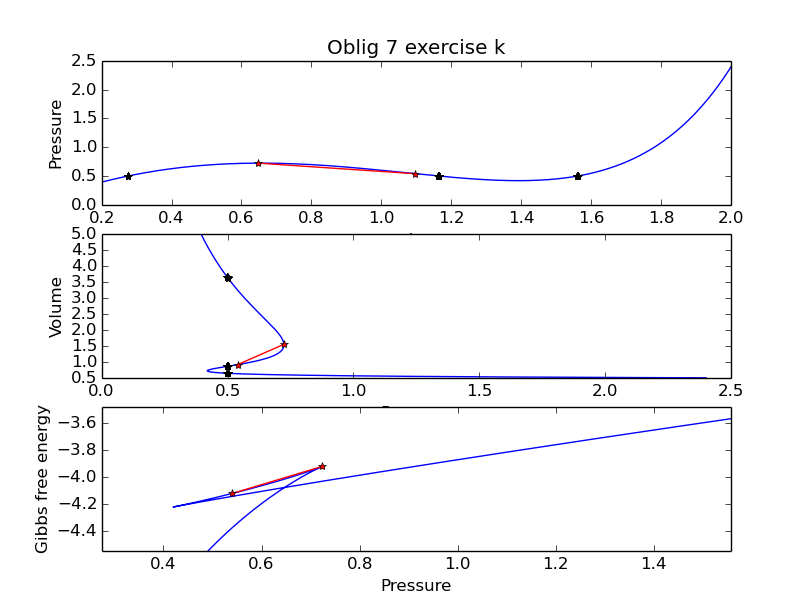
\includegraphics[scale=1]{figure_4.png}
\caption{Med test for hvor verdiene krysser hverandre}
\label{fig:4}
\end{figure}
 
\subsection*{n)}

I mellom de to krysspunktene tror jeg at systemet går fra fast til flytende og dermed får et hopp i Gibbs fri energi. 

 
\end{document}